\documentclass[10pt, a4paper]{article}
\usepackage[utf8]{inputenc}
\usepackage[UKenglish]{babel}
\usepackage{xcolor, graphicx}
\usepackage{imakeidx}
\usepackage[scale=0.85]{sourcecodepro}
\usepackage{amsmath, amssymb, amsfonts}
\usepackage{microtype}
\usepackage{comment}
\usepackage{physics}
\usepackage{siunitx}
\usepackage{tikz}
\usepackage{multicol}
\usepackage{pbalance}
\usepackage{bookmark}
\usepackage{geometry}
\usepackage[print=m, lang=fortran, verbose]{fortex}

\makeindex

\usetikzlibrary{decorations.markings}
\definecolor{fortexbg}{HTML}{F8F8F0}
\definecolor{fortextab}{HTML}{C0C0A8}
\usemintedstyle{ayu}
\setfortex{tabsize=2, breaksymbol=\scriptsize{$\hookrightarrow$}, fontsize=\small, breaklines, bgcolor=fortexbg, showtabs, tab={\rm{$\big|\hspace{0.825ex}$}}, tabcolor={fortextab}}
\DefineShortVerb{\"}

\DeclareMathOperator{\sign}{sign}

\title{Hough transforms and convolution}
\author{Henry Linton}

\begin{document}

\maketitle

Obstinately this file contains all the stuff relating to the Hough transform, however there are a few smaller functions that are used elsewhere when dealing with root data and reconstructing the data from the "root" files.

\section{exported C functions: \texttt{conv.h}}
\begin{subfile}{C}{conv.h}
\begin{code}
#ifndef CONV 
#define CONV
extern "C" {
	void init_conv();
	void a2img_orig(int *l,
	                float *x, float *y,  float *z,
	                float *sensor, float *img);
	void a2img(int *l,
	           float *x, float *y,  float *z,
	           float *img);
	void save_cur_img(int *i, int m);
	void eta_beta(double *m, double *px, double *py, double *pz,
	              double *eta, double *beta);
	void convolve();
	void find_circ_centre_orig(int *l,
	                           float *x, float *y, float *z,
	                           float *sensor, float *retval);
	void find_circ_centre(int *l,
	                      float *x, float *y, float *z,
	                      float *retval);
	void delete_conv();
}
#endif 
\end{code}
\end{subfile}

\section{Mucking around with convolutions and Hough transform}

The idea of this program is that we are going to be performing a convolutional Hough transform on some test data.

This program used FFTW3 to do the convolutions, specifically the single precision version of the library. 
one thing to not is I have no idea why but sometimes the functions are "sfftw_"... and sometimes they are "fftwf_"... And I have no idea when to use one over the other.

\begin{code}
module conv
	use ISO_C_BINDING
	use stdlib_io_npy 
	use stdlib_math 
	use writeimgf
	
	implicit none 
	include "fftw3.f03"
	
	private 
	public :: init_conv, a2img, convolve, find_circ_centre, delete_conv
\end{code}

Note that we have used the Fortran 2003 implementation of FFTW because its slightly nicer than the F77 one. 

Size of the image has been hardcoded because why not.
Here we are going to be using $128\times128\times16$ px images.  

\begin{codevar}{A_i, A_ir}
\begin{code}
	integer(c_int) :: A_i
	parameter(A_i=128)
	integer(c_int) :: A_ir
	parameter(A_ir=16)
	\end{code}
\end{codevar}

One complication is that the sensor is not actually a square. Because of hexagonal circle packing each panel is actually $1302\times555$ \si{\milli \metre} or when the panels are stiched together is it a $1:\sqrt{3}/2$ ratio. 

One thing to note is that we still need to keep our image that we are performing the hough transform over as a $128\times128$ image as performing a Fourier transform of a image that is not a power of two is \emph{much} slower. So much slower in fact that it is better to pad the image up to the next power than it is to deal with the non-square sizes. 

On my machine I measured the difference going from a $128\times109$ image to a $128\times128$ as $\sim27$\si{\second} to $\sim6.5$\si{\second}

\begin{codevar}{A_is}
\begin{code}
	integer(c_int) :: A_is(2)
	parameter(A_is=[128, 109])
	\end{code}
\end{codevar}

Here are our arrays. They come in $3\times2$ flavours.  

As the Fourier transform is an out-of-place Fourier transform. i.e. the input and output array are not the same, we have an in and out arrays. Thus we need a real input and a complex output for a forward transformation and vice-versa for a backwards.

Where $K$ is the convolution filter, and $M$ is the image that we are convolving, and $H$ is the final convolved image. 

\begin{codevar}{M_in, pm_in, M_out, pm_out, plan_m, K_in, K_out, pk_in, pk_out, plan_k, H_in, H_out, ph_in, ph_out, plan_h}
\begin{code}
	type(c_ptr) :: pm_in, pm_out, pk_in, pk_out, ph_in, ph_out
	type(c_ptr) :: plan_m, plan_k, plan_h
	real(c_float),            pointer :: M_in(:, :)
	complex(c_float_complex), pointer :: M_out(:, :)
	real(c_float),            pointer :: K_in(:, :, :)
	complex(c_float_complex), pointer :: K_out(:, :, :)
	complex(c_float_complex), pointer :: H_in(:, :, :)
	real(c_float),            pointer :: H_out(:, :, :)
	
	contains
\end{code}
\end{codevar}

\subsection{Making the circle and cone convolution filters.}

Because we are doing essentially the same convolution multiple times it makes sense for us to split of some of the precomputation work to a function that only gets executed once. 

Of these "sfftw_plan_dft_nd" is the slowest and was easily the bottleneck in the older versions of this code (to the extent that it took just under a second for a run), and with 20000 runs to do that would take a lot of time. 

We use "fftw_alloc_*" to ensure that the allocation of memeory is in a way that fftw is happy with.

Finally we precompute the Fourier transform of the convolution filter $K$ because this ony needs to be done once, so may as well do it here. 

\begin{codeblock}{init_conv}
\begin{code}
subroutine init_conv() bind (c)
	integer(c_int) :: imp_suc
	imp_suc = fftwf_import_system_wisdom()
	
	pm_in  = fftwf_alloc_real(int(A_i * A_i       , c_size_t))
	pk_in  = fftwf_alloc_real(int(A_i * A_i * A_ir, c_size_t))
	ph_out = fftwf_alloc_real(int(A_i * A_i * A_ir, c_size_t))
	
	pm_out = fftwf_alloc_complex(int((A_i/2+1) * A_i       , c_size_t))
	pk_out = fftwf_alloc_complex(int((A_i/2+1) * A_i * A_ir, c_size_t))
	ph_in  = fftwf_alloc_complex(int((A_i/2+1) * A_i * A_ir, c_size_t))
	
	call c_f_pointer(pm_in,  M_in,  [A_i, A_i      ])
	call c_f_pointer(pk_in,  K_in,  [A_i, A_i, A_ir])
	call c_f_pointer(ph_out, H_out, [A_i, A_i, A_ir])
	
	call c_f_pointer(pm_out, M_out, [A_i/2+1, A_i    ])
	call c_f_pointer(pk_out, K_out, [A_i/2+1, A_i, A_ir])
	call c_f_pointer(ph_in,  H_in,  [A_i/2+1, A_i, A_ir])

	plan_m = fftwf_plan_dft_r2c_2d(      A_i, A_i, M_in, M_out, FFTW_ESTIMATE)
	plan_k = fftwf_plan_dft_r2c_3d(A_ir, A_i, A_i, K_in, K_out, FFTW_ESTIMATE)
	plan_h = fftwf_plan_dft_c2r_3d(A_ir, A_i, A_i, H_in, H_out, FFTW_ESTIMATE)
	
	K_in = mkcone()
	
	call sfftw_execute_dft_r2c(plan_k, K_in, K_out)
	call fftw_destroy_plan(plan_k)
	call fftw_free(pk_in)
	
end subroutine
\end{code}
\end{codeblock}

Here is the implementation of the cone, it is defined over an $\text{size}(x,y,r) = A_i \times A_i \times A_i$ array. 

The main reason what we are using an convolution approach is because that is the mathematics that I am familiar with, as well as it being faster than the 3 loop approach.

Note that whilst this looks annoying with the "mod(x+A_i/2, A_i)" functions the idea is that the centre of the cone be on the corner and it rolls around to the other corners (see Figure \ref{fig:k})

\begin{figure}[h]
\centering

\includegraphics[width=0.3\textwidth]{Images/circ.png}
\caption{A slice of the cone $K$}
\label{fig:k}
\end{figure}

\begin{codeblock}{mkcone}
\begin{code}
pure function mkcone() result (retval)
	integer :: x, y, r_int 
	real(c_float), dimension(A_ir ) :: r
	real(c_float), dimension(A_i, A_i, A_ir) :: retval
	
	r = real(linspace(0, 40, A_ir), c_float)
	
	do concurrent ( y = 1:A_i, x = 1:A_i, r_int = 1:A_ir )
	
		if ( abs(   ( x - A_i/2 )**2  &
		          + ( y - A_i/2 )**2  &
		          - ( r(r_int) )**2 &
		        ) < 5 * r(r_int) ) then 
			
			retval(mod(x+A_i/2,A_i)+1, mod(y+A_i/2, A_i)+1, r_int) = 1.
		else
			retval(mod(x+A_i/2,A_i)+1, mod(y+A_i/2, A_i)+1, r_int) = 0.
		end if 
		
	end do
	
end function
\end{code}
\end{codeblock}

Because we are allocating a whole bunch of memory in "init_conv", we should deallocate it. 
Strictly speaking this is expected to only be run once right at the end, so its probs not a huge deal if it does not get run, but whatever, here it is. 

\begin{codeblock}{delete_conv}
\begin{code}
subroutine delete_conv() bind(c)
	call sfftw_destroy_plan(plan_m)
	call sfftw_destroy_plan(plan_h)
	
	call fftwf_free(pm_in)
	call fftwf_free(pm_out)
	
	call fftwf_free(pk_out)
	
	call fftwf_free(ph_in)
	call fftwf_free(ph_out)
end subroutine
\end{code}
\end{codeblock}

\section{Images from ragged arrays}

One of the big problems with the simulation data is that it does not account for the fact that multiple photons are not allowed to arrive in the same sensor. Normally fir the simulations done with this software this is not an issue as there are not that many photons. 

However because magnetic monopoles produce $\sim5000\times$ more photons than the equivalent electron this now becomes a problem. 
As such we need to remove all hits in the data that have the same $x$, $y$, and $z$ coordinates.

In the first iteration of this code I did an $O(n^2)$ approach using two loops. first one to check if it had seen the element before and the second one to increment the elements. 
This ended up being quite a big bottle neck when the lists in question are millions of elements long. 

I ended up implementing a bloom filter to deal with all these elements in $O(n)$ time instead, because all it really matters is we have order $1$ photon per pixel, not $100$. 

The number of places in the bloom filter bitfield is the number of total pixels in the sensor array $m$. this may be too few but I need to do some more testing to see if this is actually the case.

\begin{codeblock}{cln_dat}
\begin{code}
subroutine cln_dat(n, x, y, z, sensor, retval, retlen)
	integer :: m
	parameter(m = 32*32*14*14 )
	integer :: k
	parameter(k = 3)
	
	integer(c_int), intent(in)  :: n
	real(c_float),  intent(in)  :: x(n), y(n), z(n), sensor(n)
	real(c_float),  intent(out) :: retval(k, n)
	integer,        intent(out) :: retlen
	
	integer, allocatable :: h(:, :)
	logical, allocatable :: bitfield( : )
	
	integer :: i, j
	
	allocate( bitfield( m ), h(n, k)) 
	
	bitfield = .True.
	j = 0
\end{code}

Now I don't really know what hash functions I should be using for this bloom filter so I kinda just made them up. 

Hopefully this is not a problem. But the advantage of using these filters is because they are all intrinsics, it is really easy to vectorise and parallelise these, and I have checked to make sure this is the case. 

One design choice I did make was to make sure that $[0, 1]$ would not hash to the same thing as $[1, 0]$.

\begin{code}
	h(:, 1) = abs(mod( int(x) + int(y) + int(z), m ))
	h(:, 2) = abs(mod( ieor( int(x)*2 , int(y)*98 ) + int(z) , m ))
	h(:, 3) = abs(mod( ishft(int(z), 1) + ishft(int(x), -1) * int(y), m ))
	h = h + 1
\end{code}

Note that we are doing a few other filtering operations here, mainly because this is a convenient place to do it more than anything.

The first is that we only care about Rich1 not Rich2. This is represented as either $0$ or $1$ in the sensor field. Weirdly it is a floating point value so lets just use $>$ because why not. 

Second is there are occasionally some stray pixels around the origin so we just filter them out using $\lvert y \rvert < 100$. 

Finally there are sometimes some $x$ pixels outside the range and I see no pattern. 

\begin{code}
	do i = 1, n 
		if (                              &
			(any(bitfield(h(i, :))) ) .and. &
			(sensor(i) < 0.5 ) .and.        &
			(abs(y(i)) > 100 ) .and.        &
			(abs(x(i)) < 1000)              &
		) then 
			
			j = j+1
			retval(:, j) = [x(i), y(i), z(i)]
		end if 
		bitfield( h(i, :) ) = .False.
	end do 
	retlen = j
	print *, retlen
end subroutine
\end{code}
\end{codeblock}

One of the complexities is that the ROOT data does not store an image of the sensors but rather an array of arbitrary length containing all of the positions $x$, $y$, and $z$, of the hit pixels e.g. $x = {0.5, -1.2, ...}$. However the hough transform operates over images and not arrays of active points.

In order to fix this we load these arrays into a \oldstylenums{2}\textsc{d} image doing all the relevant transforms to bring from a global $x$, $y$, $z$ space into a flat image. 

\begin{codeblock}{a2img_orig}
\begin{code}
subroutine a2img_orig(l, x, y, z, sensor, d) bind(c)
	integer(c_int), intent(in)  :: l
	real(c_float),  intent(inout)  :: x(l), y(l), z(l)
	real(c_float),  intent(in)  :: sensor(l)
	real(c_float),  intent(out) :: d(A_i, A_i)
	
	integer :: l_prim
	integer, allocatable :: x_norm(:), y_norm(:)
	
	real :: tmp(3, l) 
	integer :: i, j
	real :: k
	
	d = 0
\end{code}

A bit of the code below assumes that we have at least one pixel in the input array. 
However I know for a fact that this is not always the case, so to deal with this, a simple guard statement is used. 

\begin{code}
	if (l == 0) then 
		return 
	end if 
\end{code}

Let us remove pixels that are not in rich1 and make sure that all the pixels only have 1 photon landing in them and not multiple. 

\begin{code}
	call cln_dat(l, x, y, z, sensor, tmp, l_prim)
\end{code}

Sometimes \emph{all} of the detections are in RICH2, thus after filtering we are left with no detections. So lets just return early to save computation and potential bugs. 

\begin{code}
	if (l_prim < 1) then 
		return 
	end if 
\end{code}

RICH1 at the lhcb, actually has two different detectors, one above the beampipe and one below, both of them tilted in towards the centre as shown in Figure \ref{fig:rich}.

\begin{figure}[h]
\centering
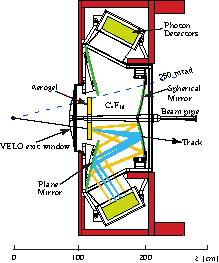
\includegraphics[width=0.3\textwidth]{Images/RICH.pdf}
\caption{Diagram of RICH1 sensor}
\label{fig:rich}
\end{figure}

As our data in coming in from a global $x$, $y$, $z$ realspace, and we need to convert this to a $x'$, $y'$ sensor space. 
The following code does this using the equation:

\begin{align}
 x' &= x \\
 y' &= 0.8866 \cdot z\ - y \cdot \sqrt{ 1 - ( 0.8866 )^2 } - 500\cdot \sign(y)   
\end{align}

Note however, that the equation provided is not quite this and the $0.8866$ constant in this equation goes to $0.8867$ on the other sensor. 
This does mean that the code is a bit messier and probs slower because of vectorisation issues, but whatever, I am just going to use the provided equation. 

\begin{code}
	associate (x => x(:l_prim), y => y(:l_prim), z => z(:l_prim))
		x = tmp(1,:)
		y = tmp(2,:)
		z = tmp(3,:)
		
		k = 970
		
		where ( y > 0 )
			y = z * (  0.8866 ) - y * sqrt( 1 - (  0.8866 )**2 ) - k
		elsewhere 
			y = z * ( -0.8867 ) - y * sqrt( 1 - ( -0.8867 )**2 ) + k
		end where
\end{code}

At the moment we still only have 2 lists of $x$ and $y$ points. But our Fourier transform requires and array.
So we normalise it to an integer position on our grid then use that as a mask to set the points to a value of 1.

\begin{equation}
x_\text{norm} = \left\lceil\frac{x - \min(x)}{\max(x) - \min(x)}\right\rceil
\label{eqn:norm}
\end{equation}

Equation \eqref{eqn:norm} is the equation to normalise all values of a matrix $x_\text{norm} \in [0, 1]$

because we want to turn these into array indices we want $x_\text{norm} \in [1, A_i]$, we need to scale it up appropriately.

\begin{code}
		allocate(x_norm(l_prim), y_norm(l_prim))
		
		print *, maxval(x), maxval(y), minval(x), minval(y)
		x_norm = ceiling((x - (-651.)) / (1302.) * (A_i -1)) + 1 
		y_norm = ceiling((y - (-555.)) / (1110.) * (109.-1)) + 1
! 		x_norm = ceiling((x - (minval(x))) / (maxval(x) - minval(x)) * (A_is(1)-1)) + 1 
! 		y_norm = ceiling((y - (minval(y))) / (maxval(y) - minval(y)) * (A_is(2)-1)) + 1
		print *, maxval(x_norm), maxval(y_norm), minval(x_norm), minval(y_norm)
	
	end associate
\end{code}

We then use these normalised points as the index for an array. This is not a very same way to do this operation as I know that sometimes an errant pixel will make it out and you then have to deal with overflows. But whatever, it is safe for the data that I am working and its not like this is a security application.  

\begin{code}
	d=0
	do concurrent(i = 1:l_prim)
		d(x_norm(i), y_norm(i)) = 1.0 + d(x_norm(i), y_norm(i))
	end do
	
	deallocate(x_norm, y_norm)
end subroutine
\end{code}
\end{codeblock}

At some point during the course, we ended up switching to a different input format where the data now comes in flat, and corrected, instead being raw positions in reals space. 
In addition the data from \textsc{rich}\oldstylenums1 is now in a different tuple from \textsc{rich}\oldstylenums2, so there is no need to filter them based on a bool array.

This means that there is now no need to do that weird correction formula, though I am still not super confident that the new images are prefect and I want to talk to McCann about it. 
This new images should be continuous over $y=0$, but they are not and need a correction of $\pm 95$ to work correctly. 

Similarly if it is corrected as I think it is, $z=0$, but this is not the case and in reality $z\in[-5,5]$. I don't know why this is the case, but it is. 

Anyway Do some quick corrections, here and load it into the image, At the moment I am not super concerned about how it looks, as long as it is \emph{somewhat} correct. 

\begin{codeblock}{a2img}
\begin{code}
subroutine a2img(l, x, y, z, d) bind(c)
	integer(c_int), intent(in)  :: l
	real(c_float),  intent(inout)  :: x(l), y(l), z(l)
	real(c_float),  intent(out) :: d(A_i, A_i)
	
	integer, allocatable :: x_norm(:), y_norm(:)
	integer :: i
	
	allocate(x_norm(l), y_norm(l))
	
	d = 0
	if (l == 0) then 
		return 
	end if 
	
	y = y - sign(95., y)
	
	x_norm = ceiling((x - (minval(x))) / (maxval(x) - minval(x)) * (A_is(1)-1)) + 1 
	y_norm = ceiling((y - (minval(y))) / (maxval(y) - minval(y)) * (A_is(2)-1)) + 1
	
	do concurrent(i = 1:l)
		d(x_norm(i), y_norm(i)) = 1.0 + d(x_norm(i), y_norm(i))
	end do
	
end subroutine
\end{code}
\end{codeblock}

\section{Interface}

This is the interface function that will be called from the "C++", at the moment it is not returning anything, but just outputting a npy file for plotting.

Here $x$ goes from $x\in[-650, 650]$ and $y$ is split between $y \in [\pm1000, \pm1300]$

\begin{codeblock}{find_circ_centre_orig}
\begin{code}
subroutine find_circ_centre_orig(l, x, y, z, sensor, retval) bind(c)
	integer(c_int), intent(in)  :: l
	real(c_float),  intent(inout)  :: x(l), y(l), z(l)
	real(c_float),  intent(in)  :: sensor(l)
	real(c_float),  intent(out) :: retval(4)
	
	call a2img_orig(l, x, y, z, sensor, M_in)
	call convolve()
	
	retval(1:3) = real(maxloc(abs(H_out)), kind=c_float)
	retval(4) = real(maxval(abs(H_out)), kind=c_float)
	
end subroutine
\end{code}
\end{codeblock}

\begin{codeblock}{find_circ_centre}
\begin{code}
subroutine find_circ_centre(l, x, y, z, retval) bind(c)
	integer(c_int), intent(in)  :: l
	real(c_float),  intent(inout)  :: x(l), y(l), z(l)
	real(c_float),  intent(out) :: retval(4)
	
	call a2img(l, x, y, z, M_in)
	call convolve()
	
	retval(1:3) = real(maxloc(abs(H_out)), kind=c_float)
	retval(4) = real(maxval(abs(H_out)), kind=c_float)
	
end subroutine
\end{code}
\end{codeblock}


And finally the function that does most of the work here: Performing the convolution of $M_\text{in}$ with the cone.

\begin{codeblock}{convolve}
\begin{code}
subroutine convolve() bind(c)
	integer :: i 
\end{code}

FFTW3 as far as I can tell doesn't have a convolution function, and so this is implementation explicitly takes the convolution as:

\begin{equation}
H(x,y) = \mathcal{F}^{-1}\big[\mathcal{F}[M(x,y)] \cdot \mathcal{F}[K(x,y)]\big]
\end{equation}

Note that we have precomputed $\mathcal{F}[K(x,y)]$ so speed it all up.
We are also only doing a \oldstylenums{2}\textsc{d} forward transformation over $M_\text{in}$ als expanding it out in Fourier space. This allows quicker computation as the complexity of a $n$\textsc{d} Fourier transform is $O(x^n \log^n(x))$. 

As of now I cannot think o fa way to avoid the second 3d convolution.

\begin{code}
	call sfftw_execute_dft_r2c(plan_m, M_in, M_out)
	
	do concurrent (i = 1:A_ir)
		H_in(:,:,i) = M_out * K_out(:,:,i)
	end do 
	
	call sfftw_execute_dft_c2r(plan_h, H_in, H_out)
	
end subroutine
\end{code}
\end{codeblock}

Some of the important mentric that can be extracted from the root file are $\eta$ and $\beta$. These can be derived from the momentum by:

\begin{align}
\eta =& \frac{1}{2} \tanh^{-1}\left( \frac{p_z}{\lvert \mathbf{p}\rvert} \right) \\
\beta =& \sqrt{\frac{\lvert \mathbf{p}\rvert ^2}{\lvert \mathbf{p}\rvert^2 + m^2}}
\end{align}

Here $\eta$ is similar to the angle of the resulting particle but is a bit of a weird measure in that parallel to the beam $\eta =0$ and perpendicular $\eta=\infty$. 

$\beta$ on the other hand is just the regular relativistic velocity.

At the moment I am assuming that the mass $m$ of the monopole is listed as "Generated_PE" in the root file. 

The lhcb and its RICH1 detectors can only use a cetain range of $\eta$ and $\beta$, so we need to figure out that are the efficiencies of the monopoles in these ranges as well as the efficiency of the algo. For the lhcb these are

\begin{align}
 2 < \eta& < 5\\
 1/n_\text{a} < \beta& < 1
\end{align}

where we are using the best case scenario of the monopole hitting the aerogel. 

\begin{codeblock}{eta_beta}
\begin{code}
subroutine eta_beta(pe, px, py, pz, eta, beta) bind(c)
	real(c_double), intent(in)  :: pe, px, py, pz
	real(c_double), intent(out) :: eta, beta
	
	real(c_double) :: p2, m2
	p2 = px**2 + py**2 + pz**2
	m2 = pe**2 - p2
	
	eta =  atanh(pz / sqrt(p2))
	beta = sqrt( p2 / (p2 + m2) )
end subroutine
\end{code}
\end{codeblock}

Just a simple function to save the current image to a numbered ppm file. This is mainly useful for just getting an understanding of the data, as well as debugging special cases like ``are there any photons in the image at all''

Note that this will happily produce images from $0-999$. but due to length restrictions, it will not go above $1000$. This is easily changed in the future though if I ever need to print over 100 images.

\begin{codeblock}{save_cur_img}
\begin{code}
subroutine save_cur_img(i, m) bind(c)
	integer(c_int), intent(in) :: i
	integer(c_int), value, intent(in) :: m 
	
	character(len=16) :: FMT
	character(len=32) :: fn
	
	write(FMT, "(A6I1A3)") "(A7I0.", m, "A4)"
	write(fn, FMT) "ns~img/", i, ".ppm"
	
	print *, "saving: ", fn 
	call writeimg(fn, M_in, [128, 128])
end subroutine
end module
\end{code}
\end{codeblock}

\printindex

\end{document}
